\documentclass[11pt,english]{article}

\setlength{\oddsidemargin}{0cm}
\setlength{\topmargin}{-2cm}
\setlength{\textwidth}{160mm}
\setlength{\textheight}{230mm}

\usepackage[english]{babel}                      
\usepackage[utf8]{inputenc}                    
\usepackage{amsmath}                             
\usepackage{amssymb}                               
\usepackage[pdftex]{graphicx}                    
\usepackage{float} 
\usepackage{subfigure} 
\usepackage[ruled,linesnumbered]{algorithm2e}
\usepackage[colorlinks, linkcolor=blue]{hyperref}
\usepackage{appendix}
\usepackage{algorithmic}
\usepackage{titletoc}
\usepackage{subcaption} % This package is used for subfigures
\usepackage{amsthm}
\newtheorem{lemma}{Lemma}
\newtheorem{definition}{Definition}

\DeclareGraphicsExtensions{.jpg,.mps,.pdf,.png}    

\usepackage{fancyhdr}

\pagestyle{fancy}
\fancyhf{} % Efface les en-têtes et pieds de page actuels
\fancyhead[C]{M1 CPA} % Texte d'en-tête
\fancyfoot[C]{\thepage}

%Sommaire en noir
\titlecontents{section}
              [0em]
              {\color{black}} % Couleur du texte
              {\bfseries\contentslabel{2.3em}}
              {\bfseries}
              {\titlerule*[1pc]{.}\bfseries\contentspage}
\hypersetup{
    colorlinks=true,
    linkcolor=black, % Couleur des liens vers des sections, sous-sections, etc.
    urlcolor=blue, % Couleur des liens URL
    citecolor=black % Couleur des liens de citation
}
\begin{document}

\title
{
    \textbf{Project CPA \\ BomberMan\\}
}

\author
{
    \\
    \\
    Submitted by
    \\
    \\
    \textbf{Haotian Xue}
    \\
    \textbf{Hejun Cao}
    \\
    M1 Science et Technologie du Logiciel 2023-2024
    \\
    Sorbonne Universite (SU UPMC)
    \\
    \\
    \\
    Under the guidance of 
    \\
    \\
    \textbf{\href{https://www-npa.lip6.fr/~buixuan/}{\textcolor{black}{Binh-Minh Bui-Xuan}}}
    \\
    Laboratoire d'Informatique de Paris 6 (LIP6)
    \\
    Centre National de la Recherche Scientifique (CNRS)
    \\
    Sorbonne Universite (SU UPMC)
}

\date{05/05/2024}

\maketitle

\begin{figure}[htbp]
    \begin{center}
        
\includegraphics[height=3cm]{./src/logo_lip6.png}
    \end{center}
\end{figure}

\begin{figure}[htbp]
    \begin{center}
        
\includegraphics[height=3cm]{./src/Science_Sorbonne_logo.png}
    \end{center}
\end{figure}

\pagebreak

\tableofcontents

\pagebreak

\large 

\section{Introduction}

\indent

Ce projet vise à utiliser Java pour implémenter les fonctions de base du jeu classique BomberMan.

\indent Dans le jeu, le personnage contrôlé par le joueur lâche une bombe qui attaquera l'ennemi avec une explosion en forme de croix après un délai. Dans le même temps, la bombe du personnage peut également détruire la boîte pour obtenir les accessoires à l'intérieur, qui peuvent être utilisés pour augmenter ou réduire la portée d'explosion de la bombe, ou pour restaurer sa propre santé.

\indent Le jeu propose un mode révolutionnaire et le but principal est de sauver la dernière princesse. Les joueurs doivent collecter des buffs dans chaque niveau, vaincre les ennemis, obtenir des clés et ouvrir la porte au niveau suivant, afin d'atteindre le dernier niveau étape par étape, trouver la princesse et la sauver.

\indent Le jeu implémente également un mode à deux joueurs. Dans ce mode, la condition de victoire du joueur est de réduire à zéro la santé d'un autre joueur.

\indent Le jeu implémente également un mode points, et la condition de victoire est d'obtenir suffisamment de points.

\indent LACK OF technologies utilisées

\indent LACK OF Gantt chart (IMAGE)


\section{Architecture}

\indent

L'architecture de ce projet est la suivante :

\begin{itemize}
    \item [$\bullet$] \textbf{package go}
    
    Ce package est principalement utilisé pour définir divers objets dans le jeu, notamment des personnages contrôlés par le joueur, des monstres, des arbres, des murs, des buffs/debuffs, et bien plus encore.
    
    En même temps, il définit également les actions individuelles du joueur/monstre. 

    Pour les joueurs, nous avons conçu son jugement de mouvement (s'il peut se déplacer dans la direction indiquée), la récupération des buffs/débuffs et la prévention des bombes.

    Pour les buffs et debuffs, nous avons mis en place une augmentation/diminution du nombre de bombes ou de la portée d'explosion.

    \item [$\bullet$] \textbf{package game}
    
    Ce package est principalement utilisé pour localiser les joueurs et les monstres, et calculer la prochaine position du joueur/monstre, ainsi que le niveau de difficulté actuel.

    \item [$\bullet$] \textbf{package engine}
    
    Il s'agit du package principal qui pilote l'implémentation du jeu. Il implémente principalement le cycle de vie de l’ensemble du jeu. Il est chargé de rafraîchir constamment tout l'écran de jeu, de charger et de mettre en œuvre l'animation (Sprite) correspondant à chaque élément, le mouvement automatique des monstres et la prédiction d'action correspondante (où apparaîtra la prochaine image).

    \item [$\bullet$] \textbf{package launcher}
    
    Ce package est principalement utilisé pour définir des cartes par défaut et charger de nouvelles cartes.

    \item [$\bullet$] \textbf{package view/audio}
    
    Ces deux packages sont principalement utilisés pour charger des images et des sons.
    

\end{itemize}

\indent Le cycle de vie principal du jeu est le suivant :

\begin{figure}[htbp]
    \begin{center}
        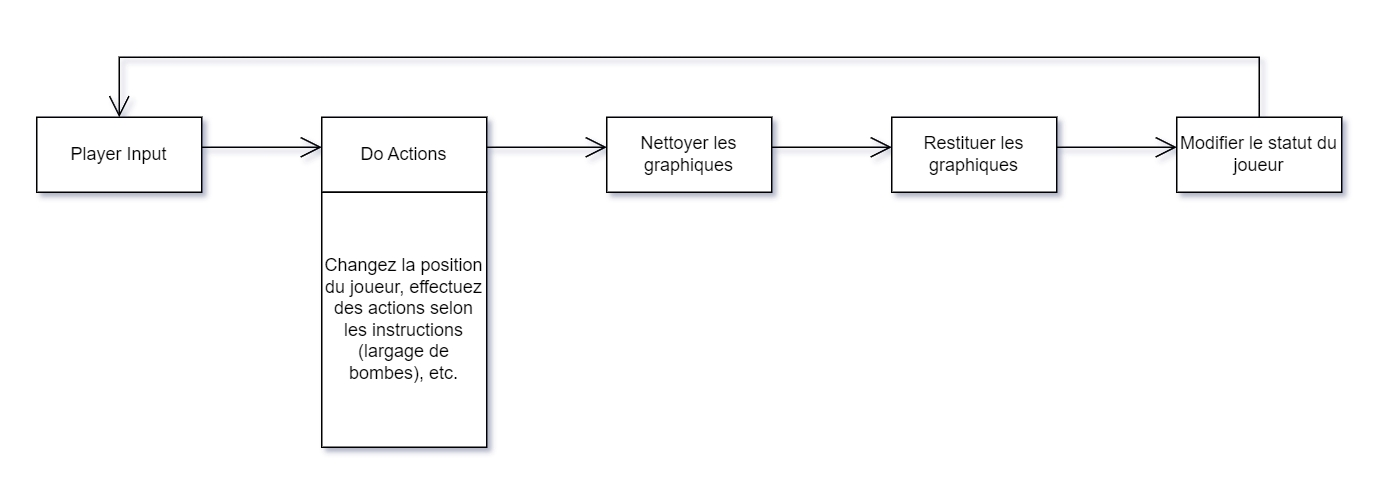
\includegraphics[height=5.5cm]{./src/cycle.png}
    \end{center}
\end{figure}

\indent De plus, afin de mieux comprendre la relation entre les Objets, j'ai dessiné le diagramme UML suivant :

\begin{figure}[H]
    \begin{center}
        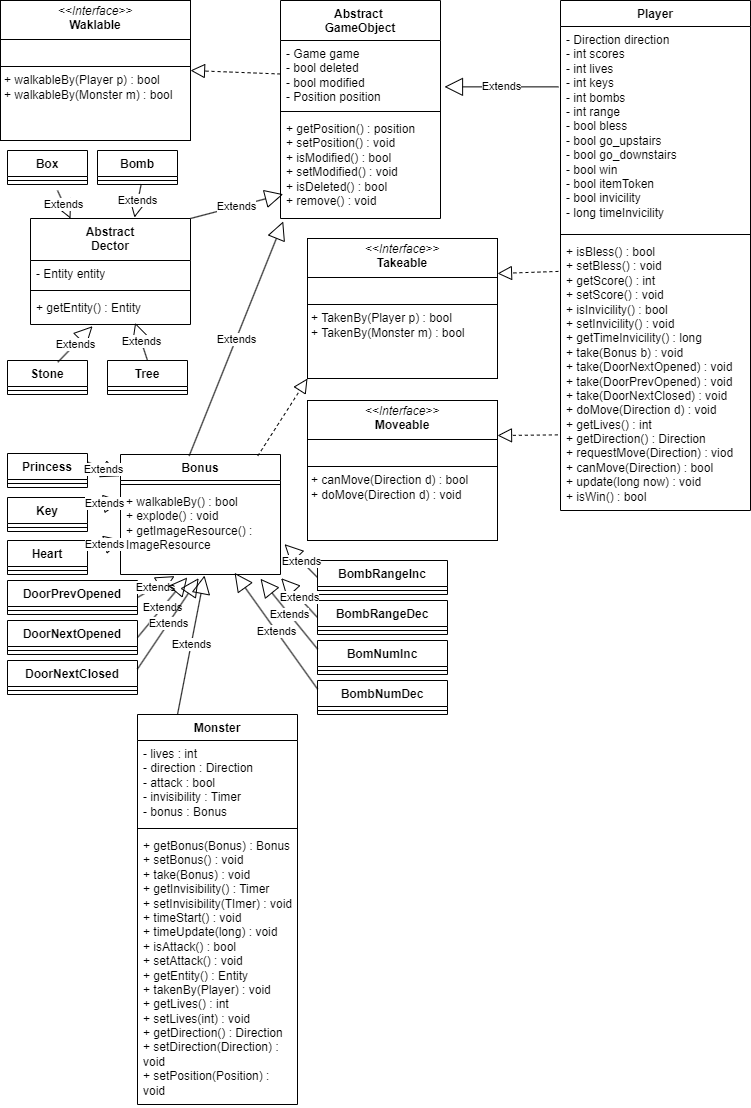
\includegraphics[height = 23cm]{./src/UML_Class.png}
    \end{center}
\end{figure}

\pagebreak

\section{Présentation Visuelle}

\indent



\section{Algorithme}

\subsection{Map Compression/Decompression}

\indent

Notre carte est en fait éditée dans un format de tableau bidimensionnel, ce qui entraînera de très sérieux problèmes de stockage car les éléments de notre carte ne sont pas très complexes et comportent de nombreux objets en double.

\indent Afin d'optimiser ce problème, nous avons conçu un algorithme de compression et de décompression pour les cartes afin de stocker et de transmettre les informations cartographiques plus efficacement.

\indent La logique de la compression de carte est la suivante :

\small
{
\begin{itemize}
    \item [$\bullet$] \textit{Step 1}
    
    Comme je l'ai dit précédemment, la carte est stockée sous la forme d'un tableau à deux dimensions. Nous parcourons donc les éléments de la carte ligne par ligne et obtenons le codage des caractères de chaque élément (via la fonction getCode), puis nous ajoutons tous ces codages à une chaîne de caractères.

    \item [$\bullet$] \textit{Step 2}
    
    Chaque fois que nous finissons de parcourir une ligne de données, nous ajoutons un "x" pour indiquer une nouvelle ligne.

    \item [$\bullet$] \textit{Step 3}
    
    Par la suite, nous utilisons un simple algorithme RLE (Run-Length Encoding) pour modifier les éléments répétés consécutifs sous forme de nombres + encodage. Par exemple, TTT (représentant trois arbres consécutifs) sera converti en 3T.

\end{itemize}
}

\large

Pour la partie décompression, c’est en fait l’inverse complet du processus de compression. Tout d'abord, la chaîne après RLE est traitée et restaurée sous la forme où un seul objet occupe un caractère, puis, sur la base du caractère de nouvelle ligne "x", le tableau bidimensionnel correspondant à la carte est construit ligne par ligne.


\subsection{IA pour Monstres}

\indent 

Dans n'importe quel jeu, les actions de l'IA de l'ennemi jouent un rôle très important, c'est pourquoi leurs algorithmes d'IA sont particulièrement importants.

\indent Puisque la seule interaction entre les monstres et les joueurs dans notre jeu est le jugement de position, la partie la plus importante est en fait la logique de recherche de chemin du monstre, qui consiste à trouver le chemin le plus court vers l'emplacement actuel du joueur.

\indent Nous avons d'abord conçu une plage de haine pour chaque monstre. Le mécanisme de recherche de chemin du monstre sera déclenché lorsque et seulement lorsque le joueur apparaîtra dans cette plage. À d'autres moments, le monstre se déplacera de manière aléatoire dans n'importe quelle direction.

\indent Quant à la recherche active du monstre, nous avons choisi l'algorithme heuristique au lieu de l'algorithme A-star, Parce que notre carte est petite, l'avantage de vitesse de l'algorithme A-star n'est pas évident. Par rapport à la simplicité de l'algorithme de recherche heuristique, l'algorithme A-star est plus difficile à mettre en œuvre.

\indent Notre conception heuristique est très simple :

\small
{
\begin{itemize}
    \item [$\bullet$] \textit{Regle 1}
    
    Si le monstre est différent du joueur sur l'axe des x, déplacez l'axe des x du monstre pour qu'il se déplace vers le joueur.

    \item [$\bullet$] \textit{Regle 2}
    
    S'il y a une différence sur l'axe y entre le monstre et le joueur, déplacez l'axe y du monstre pour qu'il se déplace vers le joueur.

    \item [$\bullet$] \textit{Regle 3}
    
    Donnez la priorité au déplacement de l’axe x du monstre.

\end{itemize}
}

\large

\section{Gestion de Collisions}

\indent

Gestion unifiée des erreurs : établissez un cadre global de gestion des exceptions pour capturer et répondre aux exceptions d'exécution dans le jeu.

\indent Journalisation détaillée : implémentez un système de journalisation pour enregistrer les opérations des utilisateurs et les erreurs système afin de faciliter le débogage et l'analyse.

\indent Nous utilisons des frameworks de journalisation tels que Log4j ou SLF4J pour mettre en œuvre des stratégies de journalisation détaillées. Ajoutez la journalisation aux points opérationnels clés, tels que la lecture et l’écriture de fichiers et les opérations utilisateur importantes.

\end{document}